% % % % % % % % % % % % % % % % % % % % % % % % % % % % % % % % % % % % % % % % % % % %
%                                                                                     %
% Short Sectioned Assignment LaTeX Template Version 1.0 (5/5/12)                      %
% This template has been downloaded from: http://www.LaTeXTemplates.com               %
%                                                                                     %
% Original author:  Frits Wenneker (http://www.howtotex.com)                          %
%                                                                                     %
% Modified by: Fco Javier Sueza Rodríguez (fcosueza@disroot.org)                      %
%                                                                                     %
% Changes:                                                                            %
%	    - Custom Chapters, Sections and Subsections (titlesec package)                %
%           - Document type scrbook (oneside)                                         %
%           - Use babel-lang-spanish package and marvosym                             %
%           - Use hyperref, enumitem, tcolorbox and glossaries packages               %
%           - Use Time New Roman (mathptmx), Helvetic and Courier fonts               %
%                                                                                     %
% License: CC BY-NC-SA 3.0 (http://creativecommons.org/licenses/by-nc-sa/3.0/)        %
%                                                                                     %
% % % % % % % % % % % % % % % % % % % % % % % % % % % % % % % % % % % % % % % % % % % %

%-----------------------------------------------%
%	              Packages                  %
%-----------------------------------------------%

\documentclass[paper=a4, fontsize=11pt, oneside]{scrbook}

% ---- Text Input/Output ----- %

\usepackage[T1]{fontenc}
\usepackage[utf8]{inputenc}
\usepackage{mathptmx}
\usepackage[scaled=.92]{helvet}
\usepackage{courier}
\usepackage[indent=12pt]{parskip}

\usepackage{geometry}
\geometry{verbose,tmargin=3cm,bmargin=3cm,lmargin=2.6cm,rmargin=2.6cm}

% ---- Language ----- %

\usepackage[spanish]{babel}
\usepackage{marvosym}

% ---- Another packages ---- %

\usepackage{amsmath,amsfonts,amsthm}
\usepackage{graphics,graphicx}
\usepackage{titlesec}
\usepackage{fancyhdr}
\usepackage{tcolorbox}
\usepackage{hyperref}
\usepackage{enumitem}
\usepackage[automake]{glossaries}

%--------------------------------------------------------------------%
%                      Customizing Document                          %
%--------------------------------------------------------------------%


% ----------- Custom Chapters, Sections and Subsections -------------- %

\titleformat{\chapter}[display]
			{\bfseries\Huge}
			{Tema \ \thechapter} {0.5ex}
			{\vspace{1ex}\centering}

\titleformat{\section}[hang]
			{\bfseries\Large}
			{\thesection}{0.5em}{}

\titleformat{\subsection}[hang]
			{\bfseries\large}
			{\thesubsection}{0.5em}{}

\titleformat{\subsubsection}[hang]
			{\bfseries\large}
			{\thesubsubsection}{0.5em}{}

\hypersetup{
    colorlinks=true,
    linkcolor=black,
    urlcolor=magenta
}

% ------------------- Custom heaaders and footers ------------------- %

\pagestyle{fancyplain}

\fancyhead[]{}
\fancyfoot[L]{}
\fancyfoot[C]{}
\fancyfoot[R]{\thepage}

\renewcommand{\headrulewidth}{0pt} % Remove header underlines
\renewcommand{\footrulewidth}{0pt} % Remove footer underlines

\setlength{\headheight}{13.6pt} % Customize the height of the header

% --------- Numbering equations, figures and tables ----------------- %

\numberwithin{equation}{section} % Number equations within sections
\numberwithin{figure}{section} % Number figures within sections
\numberwithin{table}{section} % Number tables within sections

% ------------------------ New Commands ----------------------------- %

\newcommand{\horrule}[1]{\rule{\linewidth}{#1}} % Create horizontal rule command


%----------------------------------------------------------------------------------------
%	TÍTULO Y DATOS DEL ALUMNO
%----------------------------------------------------------------------------------------

\title{
\normalfont \normalsize
\textsc{{\bfseries Curso 2023-2024} \\ Ciclo Superior de Desarrollo de Aplicaciones Web \\ IES Aguadulce} \\ [25pt]
\horrule{0.5pt} \\[0.4cm]
\huge Desarrollo de Interfaces Web \\
\horrule{0.5pt} \\[0.4cm]
}

\author{Francisco Javier Sueza Rodríguez}
\date{\normalsize\today}

%----------------------------------------------------------------------------------------
%                                     DOCUMENTO
%----------------------------------------------------------------------------------------
\makeglossaries
\loadglsentries{glossary.tex}

\begin{document}

\maketitle

\newpage

\tableofcontents

\listoffigures

%\listoftables

\newpage

\chapter{Planificación de Interfaces Web}
En este primer tema, vamos a estudiar en que consiste una interfaz web, viendo cuales son sus elementos  y las principales características que deben tener. Además, veremos conceptos básicos de diseño, haciendo hincapié en los principio de Gestalt, el color, las fuentes y otros elementos imprescindibles de una interfaz. También veremos que son las Guías de Estilo como nos pueden ayudar en el proceso de implementación de una interfaz.

\section{Elementos de Diseño}
Las personas del mundo civilizado vividos rodeadas de objetos que han sido fruto del diseño. Desde la silla donde te sientas, el microondas donde calientas la comida o la cafetera donde te haces el café. Todas y cada una de las cosas que nos rodean han pasado un proceso de diseño para lograr lo que se pretendía con su fabricación: funcionalidad, comodidad, atractivo, etc...

Utilizado normalmente en el contexto de las artes, ingeniería, arquitectura y otras disciplinas, \textbf{diseño} se define como el proceso previo de configuración mental en la búsqueda de una solución en cualquier campo.

Diseñar requiere principalmente consideraciones estéticas y funcionales. Esto necesita numerosas fase de análisis, modelado, ajustes, y adaptaciones previas a la producción definitiva del objeto. Además comprende multitud de disciplinas y oficios dependiendo del objeto que se quiere crear.

Las personas dedicadas al diseño deben comunicar sus ideas y conceptos de una forma clara y directa por medio de los elementos gráficos. La eficacia de esta comunicación dependerá de los elementos que se emplee y en conocimiento que se tenga de ellos.

\subsection{Percepción Visual}

La \textbf{percepción} es el proceso de recogida y tratamiento de la información sensorial. Consiste en recibir, a través de los sentidos las imágenes, sonidos, impresiones y sensaciones externas y elaborar e interpretar esa información.

La \textbf{percepción visual} es la sensación interior de conocimiento aparente que resulta de un estímulo o impresión luminosa registrada por nuestros ojos.

Existe una teoría (\textbf{psicología de Gestalt}) de la percepción, que estudia como nuestro cerebro decodifica la información recibida, a través de diversas asociaciones que se producen en el momento de la percepción. Según esta teoría, la mente configura, a través de ciertas leyes, los elementos que le llegan a través de los canales sensoriales o a través de la memoria.

Toda percepción es una acto de búsqueda de significado, no es recibir pasivamente la información, sino que implica buscar, seleccionar, relacionar, organizar, establecer conexiones, recordad, evaluar, etc...

En este aspecto, los diseñadores son comunicadores visuales, por lo que deben conocer al público, sus necesidades e inquietudes, para poder lograr que el mensaje visual llegue de forma correcta al receptor.

\subsection{Elementos Conceptuales: Punto, Línea, Plano y Volumen}
Los \textbf{elementos conceptuales} del diseño son la base del mismo, donde se asientan los demás elementos que veremos a continuación. Cada uno tiene sus propias características que les permite desempeñar unas funciones determinadas dentro de una composición.

\begin{itemize}
    \item \textbf{Punto}: es el resultado del primer encuentro de la punta del lápiz con el papel, tela u otro material. El \textbf{punto} es concebido en la imaginación pequeño y redondo. Un punto indica posición. No tiene largo ni ancho y es el principio y el fin de una línea y la intersección de dos líneas.

    \begin{figure}[H]
        \centering
        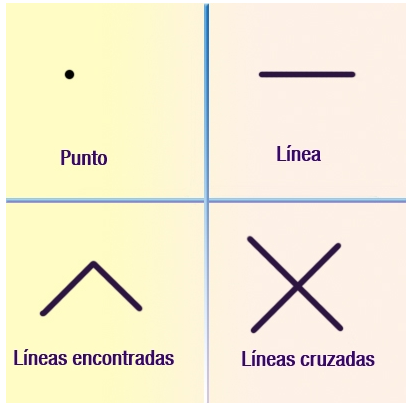
\includegraphics[scale=0.32]{el-punto.png}
    \end{figure}

    \item \textbf{Línea}: la línea no es visible por sí sola en la naturaleza. Es el resultado del movimiento de un punto que se desplaza por una superficie. La línea tiene largo pero no ancho y tiene dirección y posición. Esta limitad por dos puntos siendo esta la distancia más corta entre ambos. La línea delimita el espacio dando lugar a formas, representa el perfil o contorno de las cosas.

    \begin{figure}[H]
        \centering
        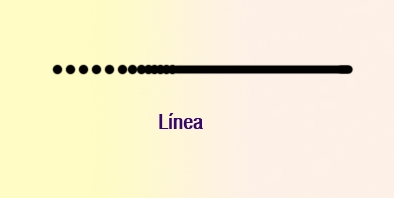
\includegraphics[scale=0.35]{la-linea.png}
    \end{figure}

    \item \textbf{Plano}: es el resultado del movimiento de una línea en dirección contraria a la suya. Un plano tiene largo y ancho pero no alto. Es la porción de superficie limitada por una línea cerrada. Define los límites extremos de un volumen.

    \begin{figure}[H]
        \centering
        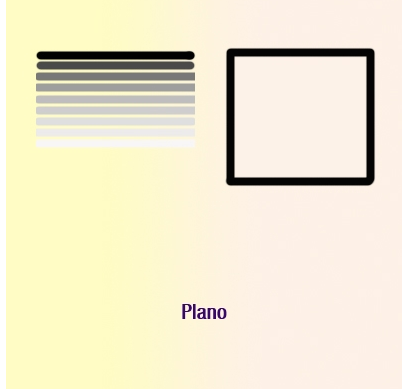
\includegraphics[scale=0.35]{el-plano.png}
    \end{figure}

    \item \textbf{Volumen}: es el resultado del movimiento de un plano que se desplaza en un dirección diferente a la suya. Tiene una posición en el espacio y esta limitado por planos. En un diseño bidimensional, el volumen es ilusorio.

    \begin{figure}[H]
        \centering
        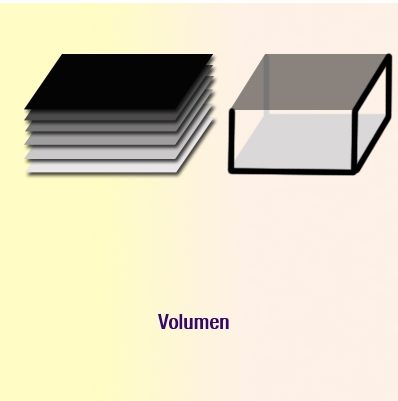
\includegraphics[scale=0.35]{el-volumen.png}
    \end{figure}
\end{itemize}

\subsection{Elementos Visuales: Forma, Medida, Color y Textura}
Los \textbf{elementos visuales} son la parte más importa de un diseño, porque son realmente lo que vemos.

Cuando dibujamos una línea en un papel empleamos una línea visible para representar la línea conceptual. Ésta tiene largo y ancho, y su color y textura vendrán determinados por el material empleado para representarla. Así, cuando lo elementos conceptuales se hacen visibles, estos tendrán color, textura, forma y medida.

\begin{itemize}
    \item \textbf{Forma}: identificamos lo que percibimos porque los que vemos posee una forma. Una forma se define como un área que se destaca del espacio que la rodea debido a un límite definido explícita o implícitamente.

    \begin{figure}[H]
        \centering
        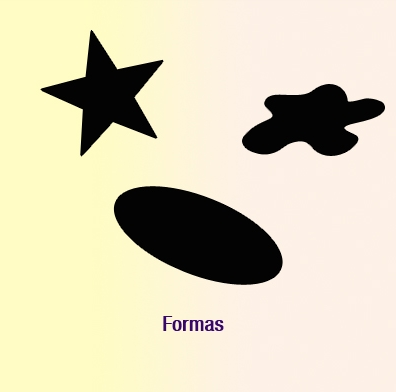
\includegraphics[scale=0.35]{la-forma.png}
    \end{figure}

    La formas pueden encontrarse entre sí de diferentes maneras:

    \begin{enumerate}[label=(\alph*)]
        \item \textbf{Distanciamiento}: ambas formas están separadas entre sí.
        \item \textbf{Toque}: si las acercamos anulamos el espacio entre ellas hasta tocarse.
        \item \textbf{Superposición}: si las acercamos aún mas, una se cruza encima de la otra.
        \item \textbf{Penetración}: igual que \textbf{(c)} pero ambas aparecen transparentes, no hay arriba y abajo y los contornos siguen siendo visibles.
        \item \textbf{Unión}: igual que \textbf{(c)} pero ambas formas quedan reunidas y se convierten en una nueva forma.
        \item \textbf{Sustracción}: cuando una forma negativa se cruza con una forma positiva.
        \item \textbf{Intersección}: igual que \textbf{(d)} pero solamente vemos la porción donde las formas se cruzan.
        \item \textbf{Coincidencia}: si acercamos las formas hasta coincidir, obtenemos una única forma.
    \end{enumerate}

    \begin{figure}[H]
        \centering
        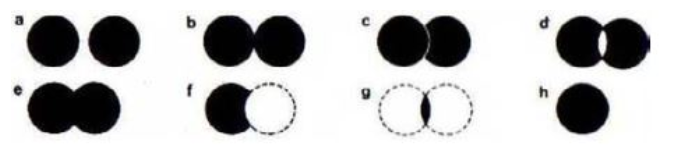
\includegraphics[scale=0.50]{la-forma-encuentro.png}
    \end{figure}

    \item \textbf{Medida}: todas las formas tienen un volumen o una dimensión. El tamaño de las formas se puede establecer de forma relativa, por comparación de unas con otras, pudiendo así decir que una forma es más grande o pequeña que otra, pero en cualquier caso, es físicamente medible.

    \begin{figure}[H]
        \centering
        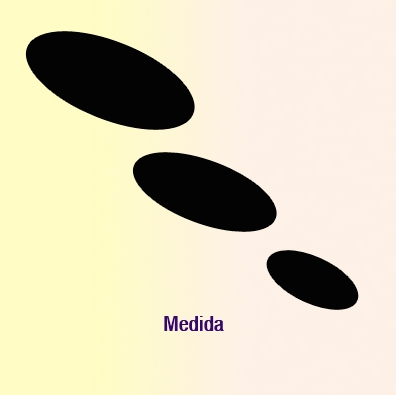
\includegraphics[scale=0.35]{la-medida.png}
    \end{figure}

    \item \textbf{Color}: todo lo que vemos en el mundo tiene color. Las cosas que vemos no solo se diferencia por su forma o tamaño, sino también por su color. El color, y el contraste de color en particular, se usa para llamar la atención sobre una parte determinada de una imagen.

    \begin{figure}[H]
        \centering
        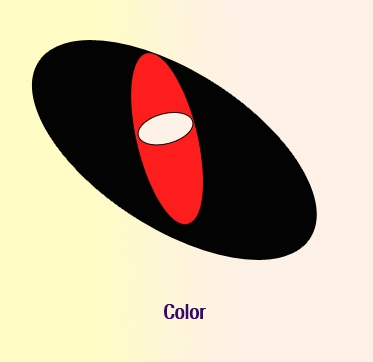
\includegraphics[scale=0.35]{el-color.png}
    \end{figure}

    \item \textbf{Textura}: es la característica visual o táctil de todas las superficies. El material con el que se hacen los objetos le aporta unas determinadas características como rugosidad, suavidad, aspereza, homogeneidad, etc...

    \begin{figure}[H]
        \centering
        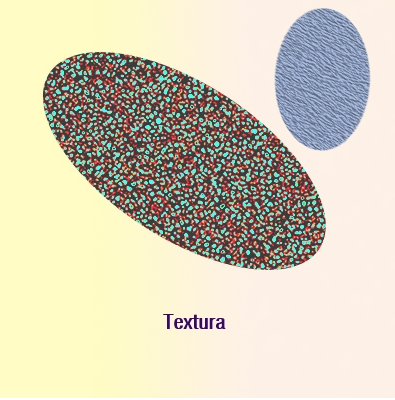
\includegraphics[scale=0.35]{la-textura.png}
    \end{figure}
\end{itemize}

\subsection{Elementos de Relación: Dirección, Posición, Espacio y Gravedad}
Este grupo de elementos gobierna la ubicación y la interrelación de las formas que componen un diseño. Algunos como la posición y la dirección pueden ser percibidos mientras que otros como el espacio o la gravedad se pueden sentir.

\begin{itemize}
    \item \textbf{Dirección}: la dirección de una forma depende de su relación con el observador, el marco que la contiene o con otras formas cercanas con cuales se compara.

    \begin{figure}[H]
        \centering
        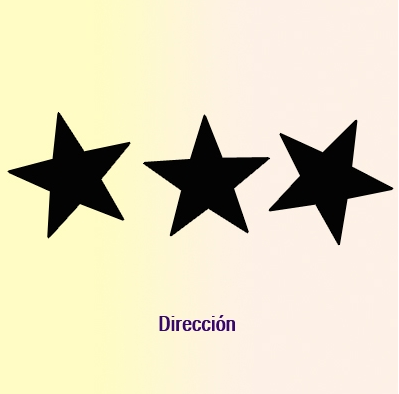
\includegraphics[scale=0.35]{la-direccion.png}
    \end{figure}

    \item \textbf{Posición}: la posición de una forma es juzgada respecto al cuadro que la contiene o la estructura global del diseño.

    \begin{figure}[H]
        \centering
        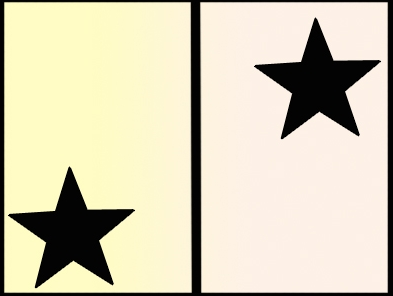
\includegraphics[scale=0.35]{la-posicion.png}
    \end{figure}

    \item \textbf{Espacio}: las formas, por muy pequeñas que sean, siempre ocupan un espacio. Así, el espacio puede estar ocupado o vacío. Se puede usar la perspectiva para simular o sugerir la ilusión de profundidad. Se pueden superponer objetos de forma que el observador perciba como más cercano el que esta delante de los demás. También podemos lograr la profundidad en el campo visual con la utilización de contraste y la variación de tamaño de las formas.

    \begin{figure}[H]
        \centering
        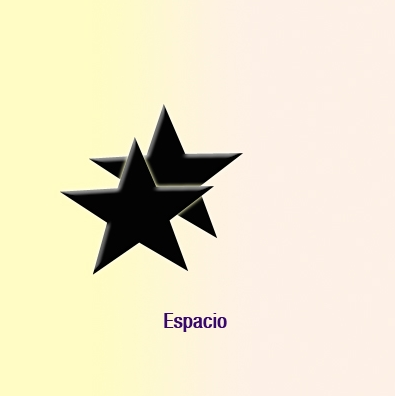
\includegraphics[scale=0.40]{el-espacio.png}
    \end{figure}

    \item \textbf{Gravedad}: la sensación de gravedad no es visual, sino psicológica. Tendemos a aplicar cualidades tales como pesadez o ligereza, estabilidad o inestabilidad, tanto a las formas individuales como a los grupos de formas.

    \begin{figure}[H]
        \centering
        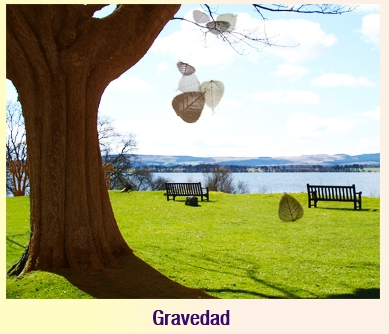
\includegraphics[scale=0.35]{la-gravedad.png}
    \end{figure}
\end{itemize}

\subsection{Elementos Prácticos: Representación, Significado y Función}
Los elementos prácticos del diseño permanecen ocultos en el contenido y la trascendencia del diseño. Estos elementos son:

\begin{itemize}
    \item \textbf{Representación}: una forma es representativa cuando se deriva del mundo natural o del mundo hecho por el ser humano. la representación puede ser \textbf{realista}, \textbf{estilizada} o \textbf{medio abstracta}. Una fotografía de un documento es una representación realista del mismo. Un dibujo de los perfiles de dicho documento es una representación estilizada. Un dibujo naif de dicho documento es una representación medio abstracta.

    \begin{figure}[H]
        \centering
        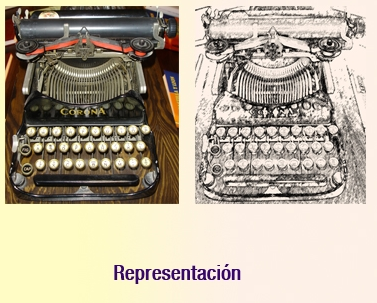
\includegraphics[scale=0.45]{la-representacion.png}
    \end{figure}

    \item \textbf{Significado}: es la imagen conceptual que se representa en nuestra mente cuando el diseño transporta un mensaje visual. Cada receptor del mensaje dará una interpretación y un significado distinto, según sean sus conocimientos y experiencias.

    \begin{figure}[H]
        \centering
        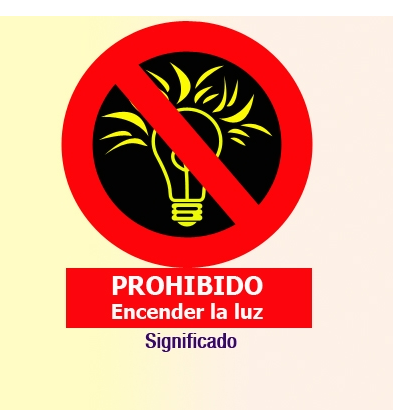
\includegraphics[scale=0.40]{el-significado.png}
    \end{figure}

    \item \textbf{Función}: la función se hace presente cuando un diseño debe servir a un determinado propósito. La imagen anterior, por ejemplo, cumple una función muy importante. Colocada en el lugar adecuado, como una sala de revelado, cumple la función de mantener el ambiente oscuro para poder trabajar.
\end{itemize}

\section{Interfaces Web}
El número de usuario de internet aumenta día a día, y el número de páginas Web también. Internet a cambiado, no solo la forma de trabajar sino también la forma en la que nos relacionamos.

Creamos páginas web para poder comunicar cosas a través de internet. Creamos páginas de tipo personal donde publicamos nuestras opiniones, nuestras fotos, nuestros viajes, etc. También creamos páginas con las que pretendemos obtener algún beneficio económico.

Todas y cada una de estas páginas son creadas con alguna finalidad. Lograr nuestro objetivo dependerá en gran medida de la eficacia del diseño que realicemos.

En \href{https://es.wikipedia.org/wiki/World_Wide_Web}{esta entrada de Wikipedia} tiene información importante que debes conocer sobre la \textbf{World Wide Web}, como su historia, estándares y tecnologías. Debes consultar también los enlaces de cada uno de los estándares.

\subsection{Interacción Persona-Ordenador}

La \textbf{IPO} (Interacción Persona-Ordenador) es la disciplina que estudia el intercambio de información entre personas y ordenadores. Cuando hay una buena interacción entre el usuario y ordenador el intercambio de información es más eficiente, hay menos errores y la satisfacción de la persona es mayor.

Hoy en día la mayor parte de los sistemas informáticos son interactivos y su éxito radica en gran medida en la eficacia del diseño de la interfaz persona-ordenador. Por ello, la interfaz debe estar diseñada pensando en las necesidades del usuario.

Debemos tener en cuenta que cada día es mayor el número de personas que utiliza el ordenador, y que estas personas se enfrentan a este tipo de interacción con diferentes niveles de formación y perspectiva.

\subsection{Diseño de una Interfaz Web: Objetivos}
Una \textbf{interfaz Web} es un \textbf{sistema gráfico} que permite a los usuarios acceder a los contenidos de la Web mediante diferentes elementos gráficos, los cuales son conocidos por la gran mayoría de usuarios que accederán a nuestra web.

El \textbf{objetivo principal} en el diseño de una interfaz Web es que sus usuarios puedan acceder a todos los contenidos de la forma más rápida y simple posible.

Para que el \textbf{diseño web} sea \textbf{efectivo}, debemos diseñar una interfaz que cobra todos nuestros objetivos. Este diseño debe facilitar que nuestros usuario puedan acceder con facilidad a todo el contenido, puedan interactuar con eficacia con todos sus componente y de forma satisfactoria.

Para conseguir dicho objetivo debemos tener en cuenta las siguiente pautas:

\begin{itemize}
    \item La paciencia de las personas no es ilimitada. Si una persona entra en una web y no encuentra rápidamente la información que esta buscando no permanecerá mucho tiempo.
    \item El gusto, considerado como una cuestión de preferencias estéticas, varia mucho de una persona a otra, pero no debemos olvidar que un diseño cuidadoso, una interfaz agradable y un uso coherente de los elementos gráficos nunca nos hará perder usuarios.
    \item Los enlaces que no funcionan o que no redirigen a la información que prometían generan en el visitante una sensación de rechazo, con la consiguiente perdida de confianza en nuestra página, llegando incluso a la determinación de no volver a visitarla de nuevo.
\end{itemize}

A la hora de \textbf{realizar el diseño} de una página web existen \textbf{diferentes filosofías} o \textbf{estrategias}. Nosotros vamos a comentar las dos más empleadas actualmente:

\begin{itemize}
    \item \textbf{Diseño Responsivo o Adaptativo}: hoy en día cuando diseñamos una aplicación debemos pensar que ésta no se va solo a visualizar en un mismo tipo de dispositivo, así que cuando la estamos diseñando tenemos que tener en cuenta los diferentes tipos de dispositivos en los que se va a visualizar. Habitualmente se desarrolla la página web primero para un ordenador y posteriormente tenemos que indicar como se va a visualizar esta en otros dispositivos como tablets, móviles, etc. Dichos cambios pueden consistir en modificar o cambiar el aspecto, o incluso en eliminar algunos elementos del diseño.

    \item \textbf{Diseño Mobile First}: actualmente esta cambiando la tendencia sobre visualización de contenido web, y mientras durante mucho tiempo las webs se han visualizado el ordenador como dispositivo principal, actualmente son los dispositivos móviles donde más páginas web se ven. Teniendo en cuenta esto, lo que persigue esta filosofía es realizar el diseño primero para un dispositivo móvil y posteriormente realizar las modificaciones oportunas para que se adapte a otro tipo de dispositivos como ordenadores.
\end{itemize}

\subsection{Características: Usable, Visual, Educativa y Actualizada}
Cuando diseñamos una web, debemos tener en cuenta como siente o como perciben los seres humanos. Si, por ejemplo, nuestra web ofrece cursillos a las personas de la tercera edad, debemos tener en cuenta las limitaciones que pueden tener este grupo de personas, como problemas de visión y audición. Mientras que si nuestro sitio web va enfocado al público infantil deberemos cuidar más la decoración e incluso abusar de colores llamativos.

Hay características que son deseables en un sitio web y características que son imprescindibles. Determinar cuales son deseable y cuales imprescindibles dependerá en gran medida del público al que vaya dirigido nuestro sitio web, aunque unas de las características que deberíamos considerar siempre imprescindibles es \textbf{la usabilidad}.

\textbf{Usable} es un termino ampliamente utilizado en el mundo informático. Es una traducción del termino inglés ``Useable'' y por analogía con el termino español ``utilizable'' podemos definirlo como ``\textbf{que se puede usar}''. Podríamos pensar que un sitio web es usable simplemente por poder acceder a él y haber visitado alguno de sus enlaces. Pero nada más lejos de la realizar, un \textbf{sitio we es usable} si al usuario le resulta \textbf{fácil} el \textbf{uso de su interfaz}.

La popularidad de un sitio web depende en gran parte de su aspecto visual. Podemos decir que un sitio web es visual cuando las percepciones del usuario, sus opiniones acerca del sitio, y sus sentimientos y actitudes generados mientras lo usa, son positivos. Un \textbf{sitio web debe ser atractivo} para mantener la atención del usuario, pero también debe ser coherente en el uso de los elementos gráficos.

Un sitio web \textbf{es visual} cuando los elementos gráficos empleados están orientados a conseguir los objetivos del sitio y no se han empleado como elementos decorativos.

Tenemos además que tener en cuenta que las personas desarrollan modelos como resultado de sus experiencias y emplean estos modelos para almacenar información y conocimiento. Una interfaz \textbf{es educativa} cuando es fácil de aprender por el usuario. La \textbf{facilidad de aprendizaje} es una medida de la \textbf{cantidad de tiempo} necesaria para \textbf{conocer la interfaz} a través de su uso y, también es una medida de la cantidad de tiempo que el usuario \textbf{retiene ese conocimiento} sin necesidad de usar la interfaz.

Si no queremos perder popularidad entre nuestro visitantes habituales, es conveniente ofrecer periódicamente nuevos contenidos que le puedan interesar. Es importante \textbf{actualizar periódicamente} nuestro sitio Web. Podemos actualizarlo diariamente, semanalmente, mensualmente, etc. Dependerá del sitio web y los servicios que ofrezcan. Pero también es importante \textbf{actualizar la interfaz} modificando aquellos elementos que puedan lograr que sea aún más usable, visual y educativa.

\subsection{Componentes de Una Interfaz Web}
Dado que la interfaz Web es el medio de comunicación entre los usuarios y el sitio web que visitan, debemos tener claros cuales son los elementos que compondrán nuestra interfaz. Todos elementos deberán permitir al usuario identificar la función que desempeñan de forma que pueda acceder a todos los contenidos sin tener que realizar extraños razonamientos.

Son muchos los elementos de los que pueda estar compuesta nuestra interfaz Web. El número de elementos utilizados dependerá de la finalidad del sitio. Así, un portal de noticias o de un organismo oficial usarán más elementos que el sitio de un restaurante o una página web personal. Los \textbf{elementos} más destacados que podemos encontrar en cualquier de ellos son:

\begin{itemize}
    \item Elementos de \textbf{Identificación}: son aquellos elementos que identifican plenamente el sitio Web. El usuario, a la vista de estos elementos, debe saber a quién pertenece la web. Por ejemplo, el logo de la página, el título de ésta, etc...
    \item Elementos de \textbf{Navegación}: son aquellos que están presentes en cada una de las pantallas de un sitio web y permiten al usuario moverse por las diferentes secciones del sitio y retomar de nuevo la portada. Estos elementos deben ser lo suficientemente intuitivos para que el usuario sepa que hay que hacer para acceder al contenido. Un ejemplo son los diferentes enlaces del sitio, barras de navegación, etc...
    \item Elementos de \textbf{Contenidos}: son las zonas en las que se muestra la información relevante de cada una de las páginas que componen el sitio. Dentro de una zona de contenido se debe distinguir la zona del Título del Contenido y el Contenido propiamente dicho. Por ejemplo, una noticia, una entrada de un blog, etc...
    \item Elementos de \textbf{Interacción}: son las zonas del sitio Web donde se ofrece la realización de acciones a los usuarios. Ejemplos son las barras de búsqueda, los formularios, etc...
\end{itemize}

\subsubsection{Zona de Navegación}
Como hemos dicho, los elementos de navegación son los que nos permiten acceder a todos los contenidos que se encuentran en las diferentes páginas que componen el sitio Web. Pero lo que no hemos dicho, es que si queremos que nuestra Web sea usable, el usuario debe conseguir poder navegar por la página sin perderse. Para conseguirlo, el sistema de navegación debería tener los siguiente elementos:

\begin{itemize}
    \item Elementos de \textbf{regreso a la portada}.
    \item \textbf{Menú de secciones} o de áreas de interés.
    \item \textbf{Información} sobre la \textbf{ubicación del usuario} dentro de sitio.
\end{itemize}

Es importante para el usuario tener algún \textbf{elemento} que le permita \textbf{volver al principio} sin necesidad de usar la herramienta ``ir hacia atrás'' del navegador. Es problema suele resolverse \textbf{empleando un enlace} en el \textbf{logotipo} de la empresa que se sitúa normalmente en la parte superior izquierda de cada una de las páginas que componen el sitio.

El \textbf{menú de secciones} es una zona de la interfaz donde se detallan las secciones y/o áreas en las que está dividida la información contenida en el sitio Web. Debe ser fácilmente localizable y se suele ubicar en la parte superior de cada página, debajo del logotipo. Es importante que estas secciones estén bien identificadas mediante un texto o imagen descriptiva. También es importante que mantenga la posición en todas las páginas que componen el sitio.

No debemos olvidar que cuando el sitio Web es suficientemente grande, con muchas secciones y subsecciones, es de gran importante que el \textbf{usuario sepa} en todo momento el lugar en el que se encuentra dentro del sitio. Por ello debemos informar, en cada una de las páginas de contenido, el camino recorrido desde la página principal hasta la página actual, y lo haremos mediante una línea de texto por encima del menú de secciones o de la zona de contenidos. Podemos aprovechar esta línea para permitir, mediante el uso de enlaces, vueltas hacia atrás en el camino de navegación. Esto es lo que se denomina como técnica de navegación de \textbf{migas de pan} o \textbf{breadcrumb}.

En la siguiente imagen, podemos ver los diferentes elementos que acabamos de mencionar en la Web del Ministerio de Educación y Ciencia.

\begin{figure}[H]
    \centering
    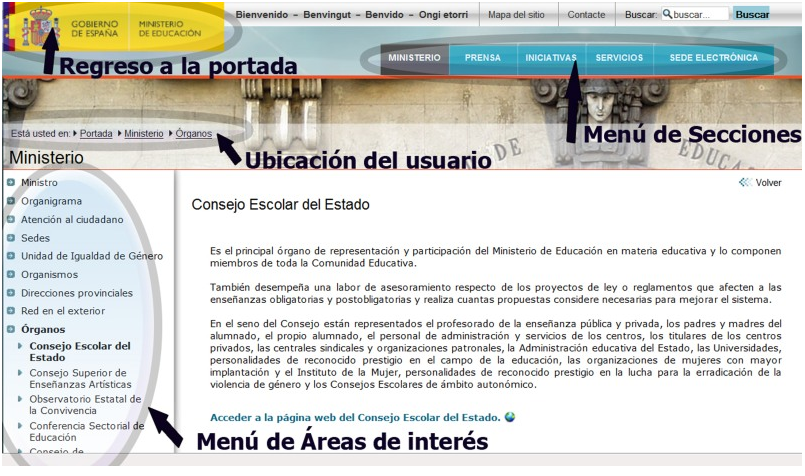
\includegraphics[scale=0.45]{elementos-navegacion.png}
    \caption{Elementos de navegación}
\end{figure}

\subsubsection{Zona de Contenido e Interacción}
El \textbf{contenido} es la \textbf{parte esencial} de una página Web. Es importante que los contenidos estén escritos en un lenguaje claro y conciso, y presentados en un formato agradable y de fácil lectura. Además, si el sitio Web esta formado por diferentes páginas, el contenido debe situarse siempre en la misma posición. También es importante evitar que el usuario tenga que realizar grandes desplazamientos durante la lectura o visualización del contenido. Siempre es mejor dividir el contenido en varias páginas y enlazar una con otra.

Cuando el usuario está navegando por un sitio Web y eligiendo los enlaces que quiere visitar de la página web está interactuando con ésta, pero no es a este tipo de interacción al que nos referimos, sino que nos referimos a otras \textbf{zonas de interacción} donde el usuario \textbf{participa} de alguna manera. Cuando el usuario selecciona el idioma en el que quiere ver la página, realiza una búsqueda usando un formulario, cuando envía una opinión o cuando firma un libro de visitas. Todos los elementos del sitio necesarios para la realización de este tipo de acciones forman parte de la \textbf{zona de interacción}.

En la siguiente imagen imagen podemos ver la misma Web de la figura anterior con las zonas de contenido e interacciones señaladas.

\begin{figure}[H]
    \centering
    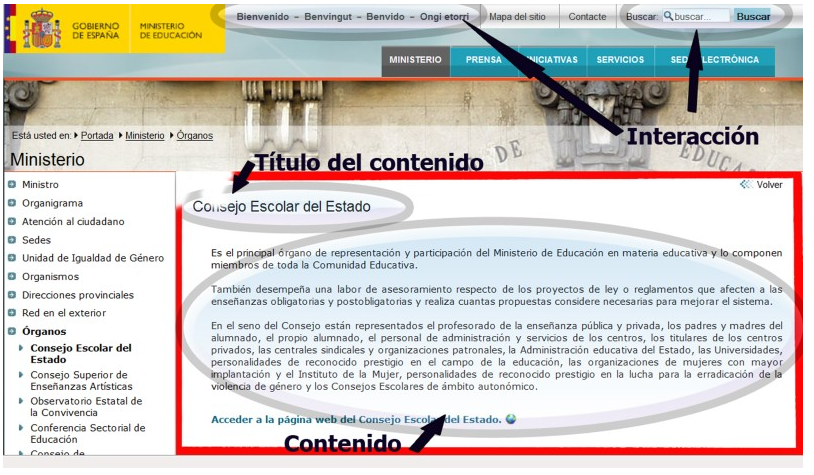
\includegraphics[scale=0.45]{elementos-contenido.png}
    \caption{Elementos de contenido e interacción}
\end{figure}

Hay muchos \textbf{elementos que permiten la interacción} y cada uno de ellos cumple una función muy concreta. Algunos de ellos son los siguientes:

\begin{itemize}
    \item \textbf{Botón}: elemento que permite al usuario realizar una acción. Se puede usar para su representación un rectángulo con efecto de relieve y con un texto que sirve para orientar al usuario sobre la función de dicho botón. Su diseño debe mantenerse en todo el sitio web.

    \item \textbf{Áreas de Texto}: son rectángulos en los que el usuario puede escribir. Deben ir acompañados de una etiqueta que indique el contenido que se le pide al usuario.

    \item \textbf{Botones de Opción}: son elementos excluyentes entre sí que están agrupados bajo una misma descripción. Constan de unas circunferencias acompañadas de un texto descriptivo. Se identifica el que esta seleccionado porque tiene un círculo negro.

    \item \textbf{Casillas de Verificación}: al contrario que los botones de opción, estás no son excluyentes entre sí. El usuario puede no seleccionar ninguna o seleccionar una, alguna o todas las casillas. Suelen ir también agrupadas bajo una misma descripción y acompañadas de un texto descriptivo. Tienen forma de cuadrado y cuando se seleccionan se marcan con una ``X'' o una ``V''.
\end{itemize}

\subsection{Maquetación Web}
Según la RAE, una \textbf{maqueta} es un boceto previo a la composición de un texto que se va a publicar, usado para determinar sus características definitivas. También define un \textbf{boceto} como esquema o proyecto en el que se bosqueja cualquier obra.

A la hora de realizar la maquetación web debemos tener en cuenta:

\begin{itemize}
    \item Cuáles son \textbf{los elementos} que van a contener cada página de nuestro sitio Web.
    \item Como irán \textbf{colocados} cada uno de esos elementos dentro de de las páginas teniendo en cuenta siempre el espacio disponible, es decir, la ventana del navegador.
\end{itemize}

Si hemos hablado con el cliente tendremos los datos necesarios para la realizar una serie de bocetos preliminares de lo que será nuestro sitio web. Además, hay que tener en cuenta, que un boceto también refleja la \textbf{interactividad} y \textbf{funcionalidad} del sitio Web.

Para \textbf{diseñar un sitio Web} debemos comentar realizan una distribución de los grandes bloques de elementos de información. Se debe tener en cuenta en el diseño a todas las páginas web que componen el sitio. Todas deben manejar la misma estructura. Este tema los volveremos a ver al final de esta unidad cuando hablemos de las plantillas de diseño.

\subsubsection{Elementos de Ordenación}
Cuando diseñamos una web debemos de ser consistentes en las distribución de los grandes bloques de información en todas las páginas que componen el sitio Web, teniendo además en cuenta el espacio disponible en la ventana del navegador.

Además de los bloques que hemos visto ya, como las zonas de navegación, contenido e interacción, podemos encontrar otros bloques, los cuales podemos ver en la siguiente figura.

En ella podemos ver un boceto de la colocación de los diferentes bloques de información. A continuación, explicaremos un poco sobre cada uno de ellos haciendo especial hincapié en los que aun no hemos comentado en puntos anteriores.

\begin{figure}[H]
    \centering
    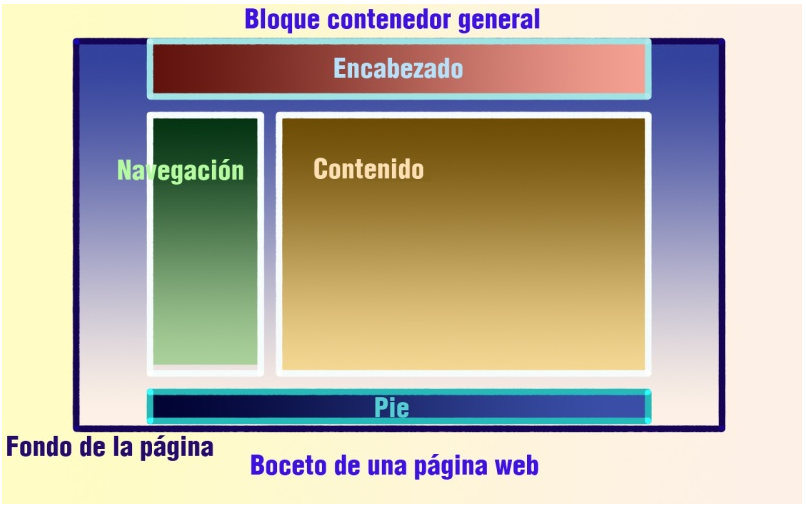
\includegraphics[scale=0.45]{boceto-bloques.png}
    \caption{Elementos de Ordenación}
\end{figure}

El \textbf{Bloque de Encabezado} esta siempre situado en la parte superior de cualquier página. Suele contener además de los elementos identificativos de la página web: el logotipo, nombre de la empresa, elementos de acción que permiten cambiar el idioma de lectura, realización de búsquedas, e incluso si el sitio es grande, elementos de navegación que permanecen a la vista en todas las páginas. Éste se \textbf{repite en todas las páginas} del sitio Web y debe ser visible en todas ellas siempre que sea posible y la complejidad del sitio nos lo permita.

El \textbf{Bloque de Navegación} es donde se coloca el sistema de navegación del que ya hemos hablado en el apartado  de Zonas de Navegación e Interacción.

El \textbf{Bloque de Contenido} es aquel en el que se muestran los contenidos. Los contenido representan la meta del usuario y la razón por la que visita nuestro sitio Web, por lo que debemos prestar mucha atención al diseño de este bloque. Debemos reservar una zona lo suficientemente grande como para que el usuario pueda leer el contenido cómodamente, sin necesidad de realizar grandes desplazamientos. Es \textbf{importantísimo} que el usuario \textbf{no tenga} que realizar \textbf{desplazamientos horizontales} para leer el final de cada línea.

El \textbf{Bloque de Pie de Página} esta situado al final de la página y al igual que en encabezado se suele repetir en todas las páginas del sitio Web. Normalmente se emplea como zona de \textbf{navegación complementaria} a la zona superior situada en el encabezado. En ellas se suelen repetir algunos enlaces que se colocan en el encabeza como Mapa del sitio del web. o el enlace de información de contacto, y además, se colocan algunos enlaces nuevos como las información relativa a los derechos de autor, privacidad, información lega, etc...

El diseño del pie no suele ser tan elaborado como el encabezado, ya que si importancia es menor. El usuario debe ser consciente que lo que está viendo es el pie. Esto es de especial importancia en aquellos casos en los que por ser el tamaño vertical de la página mayor que la ventana del navegador, el usuario se ve obligado a desplazarse verticalmente, pudiendo perder de vista el encabezado. Con un diseño más sencillo del pie respecto del resto de bloques conseguimos esa percepción por parte del usuario.

\subsection{Mapa de Navegación}
Cuando un sitio es muy grande y complejo, conviene tener un mapa del sitio que ayude a los usuarios a encontrar lo que buscan.
% Bibliography

\addcontentsline{toc}{chapter}{Bibliografía}
\bibliography{citas}
\bibliographystyle{unsrt}

\end{document}